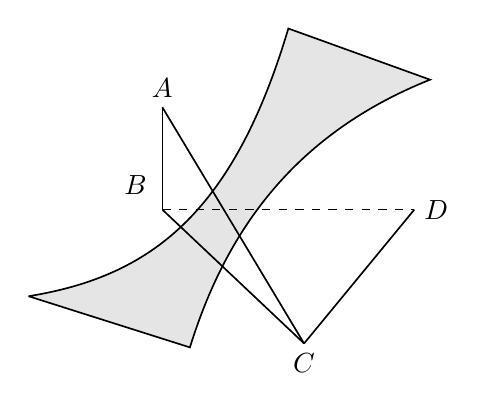
\begin{tikzpicture}[x=1cm,y=1cm,line width=.6pt,font=\normalsize]
% A continuous river strip; its two banks do not meet.
\fill[gray!20] (-1.7,-.9)--(.35,-1.55)
 .. controls (.8,-.1) and (1.65,1.15) .. (3.4,1.85)
 --(1.6,2.5) .. controls (.9,.15) and (-.15,-.65) .. (-1.7,-.9)--cycle;
\draw (-1.7,-.9)--(.35,-1.55)
 .. controls (.8,-.1) and (1.65,1.15) .. (3.4,1.85)--(1.6,2.5)
 .. controls (.9,.15) and (-.15,-.65) .. (-1.7,-.9);
% construction: AB vertical, BD dashed, BC / AC / CD solid
\coordinate (A) at (0,1.5);
\coordinate (B) at (0,0.2);
\coordinate (D) at (3.2,0.2);
\coordinate (C) at (1.8,-1.5);
\draw (A)--(B);
\draw (B)--(C);
\draw (A)--(C);
\draw (C)--(D);
\draw[dashed] (B)--(D);
% labels adjacent to points, clear of lines
\node[above] at (A) {$A$};
\node[above left=2pt] at (B) {$B$};
\node[right] at (D) {$D$};
\node[below] at (C) {$C$};
\end{tikzpicture}
